\section{Contamination Analysis}
\label{app:contamination}
\subsection{Contamination Detection Protocol}


To ensure the integrity of our evaluation, we implemented a comprehensive decontamination protocol to measure the overlap between our training dataset and all evaluation benchmarks we report results on. This protocol consists of three main stages: Index Construction, Dataset Scanning, and Leakage Reporting.

\subsubsection{Index Construction}
The first stage creates a compact, indexed set of unique n-grams from all benchmark evaluation data.

\begin{enumerate}
    \item \textbf{Text Normalization:} All text from the benchmarks is processed through a  normalization pipeline, similar to ~\cite{NEURIPS2022_ce9e92e3}: (1) Unicode normalization (NFKC), (2) conversion to lowercase, (3) tokenization, and (4) removal of a predefined list of common English stop words. This procedure focuses the resulting n-grams on substantive content.
    
    \item \textbf{N-gramming and Filtering:} We generate 13-grams, a common n-gram size for this task~\cite{brown2020language, gao2020pile} from the normalized token lists. As in~\cite{NEURIPS2022_ce9e92e3}, a set of regular expressions is used to filter out common boilerplate, exam instructions, and formatting artifacts.

     \item \textbf{Train/Test De-duplication:} as in~\cite{gao2020pile}, we compute the set of all 13-gram hashes from the \texttt{train} split and subtract this set from the 13-gram hashes generated from the \texttt{test} split. This ensures our index only contains n-grams that are unique to the evaluation set.
\end{enumerate}
\subsubsection{Dataset Scanning}
The second stage analyzes the target training dataset against the generated index.

\begin{enumerate}
    \item \textbf{Document Processing:} Each document in the training dataset is processed using the \textit{exact same} normalization, 13-gramming, and hashing pipeline used for index construction.
    
    \item \textbf{Contamination Criteria:} A document is flagged as "contaminated" if it meets two criteria, based on the set intersection of its n-gram hashes with the benchmark index:
    \begin{itemize}
        \item \textbf{Minimum Hits:} The number of distinct matching n-grams is $\geq 3$.
        \item \textbf{Minimum Coverage:} As proposed in~\cite{rae2022scalinglanguagemodelsmethods}, the coverage of matching n-grams is $\geq 0.1\%$. Coverage is defined as:
        $$
        \text{Coverage} = \frac{\text{distinct\_hits}}{\text{total\_unique\_13grams\_in\_doc}}
        $$
    \end{itemize}
\end{enumerate}

\subsubsection{Leakage Reporting}
The final stage aggregates the scan results into a summary report.

\begin{enumerate}
    \item \textbf{Numerator (Leaked N-grams):} The procedure aggregates the reports from all scanned partitions. It performs a global \textit{set union} to find all unique n-gram hashes that were found \textit{at least once} in the target dataset, aggregated by benchmark source. This provides the $\text{unique\_ngrams\_leaked}$ count for each benchmark.
    
    \item \textbf{Denominator (Total N-grams):} The procedure retrieves the pre-computed metadata to obtain the total unique n-gram count for each benchmark.
    
    \item \textbf{Final Metric:} As proposed in~\cite{touvron2023llamaopenefficientfoundation}, the \textbf{Leak Percentage} for each benchmark is then calculated as:
    $$
    \text{Leak Percentage} = \frac{\text{unique\_ngrams\_leaked}_{\text{benchmark}}}{\text{total\_unique\_ngrams\_in\_index}_{\text{benchmark}}} \times 100
    $$
\end{enumerate}

\subsection{Contamination Report}
\label{app:contam_report}

We executed our 13-gram contamination scan across the entire \num{345697271} documents of the \MixtureVitae{} dataset. The global summary of contaminated documents per benchmark is presented in Table~\ref{tab:global_contam_summary}.

The results confirm that for the vast majority of benchmarks—including ARC, HellaSwag, LAMBADA, OpenBookQA, and PIQA—the document-level contamination rate is negligible (at or below 0.0003\%), strongly validating the integrity of our evaluation on these tasks.

The scan did, however, flag a minor overlap for MMLU (0.0098\%) and BoolQ (0.0087\%), and a more significant overlap for our key code benchmarks: HumanEval (0.0988\%) and MBPP (0.0878\%). This overlap in code benchmarks is a known challenge when including large-scale permissive code corpora like The Stack, which may naturally contain snippets of common coding problems (a "source overlap" rather than a direct "test-set leak").

To ensure this overlap did not artificially inflate our model's strong performance on these key tasks, we conducted case studies for the benchmarks with the highest overlap. This analysis is detailed in the following section (Appendix~\ref{app:decontam_gsm8k}).


\begin{table}[htb]
\caption{Global contamination summary by document count, based on a 13-gram overlap scan.
This table shows the total number of documents in \MixtureVitae{} that contained
at least one overlapping n-gram from each benchmark's test set.
The total documents in \MixtureVitae{} is \num{345697271} and the overall contamination rate is 0.1420\%.}
\centering
\begin{tabular}{lrr}
\toprule
Benchmark & {Contaminated Docs} & {Contamination Rate (\%)} \\
\midrule
ALERT         & \num{12}      & 0.0000\% \\
ARC           & \num{17}      & 0.0000\% \\
BoolQ         & \num{30144}   & 0.0087\% \\
CommonSenseQA          & \num{0}    & 0.0000\% \\
GPQA          & \num{1077}    & 0.0003\% \\
GSM8K         & \num{230}     & 0.0001\% \\
HellaSwag     & \num{186}     & 0.0001\% \\
HumanEval     & \num{341554}  & 0.0988\% \\
IfEval        & \num{756}     & 0.0002\% \\
LAMBADA       & \num{23}      & 0.0000\% \\
MBPP          & \num{303558}  & 0.0878\% \\
MMLU          & \num{33922}   & 0.0098\% \\
OpenBookQA    & \num{60}      & 0.0000\% \\
PIQA          & \num{5}       & 0.0000\% \\
SimpleQA      & \num{98}      & 0.0000\% \\
\bottomrule
\end{tabular}

\label{tab:global_contam_summary}
\end{table}

\subsection{Decontaminated Test Set Performance}
\label{app:decontam_gsm8k}
To understand how test data leakage affects final performance on downstream tasks, we conducted the following experiment on all models and benchmarks reported in Section~\ref{sec:instruct_results}:
\begin{enumerate}
    \item Identify problems from the test set that have at least one 13-gram match in the training dataset.
    \item Evaluate the model on a decontaminated benchmark version obtained by removing problems that were identified.
\end{enumerate}

\begin{table*}[htb]
\caption{Validating math, code, and instruction performance by comparing original (Orig) vs.\ decontaminated (Decont) test sets for 1.7B models trained for 300B tokens. \MixtureVitae{}'s high scores are shown to be genuine, as performance is maintained after removing all overlapping test items. This confirms the model's capabilities are not an artifact of test set leakage.}
\centering
%\caption{Performance on original vs.\ decontaminated benchmarks. Metrics: GSM8K/CoT = exact\_match (flexible\_extract), MBPP/MBPP+ = pass@1, IFEval = prompt\_level\_strict\_accuracy.}
%\setlength{\tabcolsep}{6pt}
%\renewcommand{\arraystretch}{1.15}
\resizebox{\linewidth}{!}{
\begin{tabular}{l
                *{2}{c}
                *{2}{c}
                *{2}{c}
                *{2}{c}
                *{2}{c}}
\toprule
\multirow{2}{*}{\textbf{Training Dataset}} 
% --- REORDERED HEADERS (1, 4, 2, 5, 3) ---
& \multicolumn{2}{c}{\textbf{GSM8K}} 
& \multicolumn{2}{c}{\textbf{GSM8K-CoT}} 
& \multicolumn{2}{c}{\textbf{MBPP}} 
& \multicolumn{2}{c}{\textbf{MBPP+}} 
& \multicolumn{2}{c}{\textbf{IFEval}} \\
\cmidrule(lr){2-3}\cmidrule(lr){4-5}\cmidrule(lr){6-7}\cmidrule(lr){8-9}\cmidrule(lr){10-11}
& \textbf{Orig} & \textbf{Decont} 
& \textbf{Orig} & \textbf{Decont} 
& \textbf{Orig} & \textbf{Decont} 
& \textbf{Orig} & \textbf{Decont} 
& \textbf{Orig} & \textbf{Decont} \\
\midrule
\textbf{\MixtureVitae{}}     & 0.53 & 0.54 & 0.50 & 0.50 & 0.38 & 0.38 & 0.55 & 0.59 & 0.19 & 0.23 \\
SmolLM2          & 0.30 & 0.30 & 0.28 & 0.29 & 0.35 & 0.35 & 0.48 & 0.48 & 0.17 & 0.20 \\
Comma-0.1        & 0.06 & 0.06 & 0.09 & 0.09 & 0.21 & 0.23 & 0.28 & 0.28 & 0.18 & 0.20 \\
CommonCorpus-Eng & 0.02 & 0.01 & 0.01 & 0.01 & 0.02 & 0.02 & 0.04 & 0.05 & 0.12 & 0.16 \\
C4               & 0.01 & 0.01 & 0.01 & 0.02 & 0.00 & 0.00 & 0.00 & 0.00 & 0.20 & 0.21 \\
DCLM             & 0.01 & 0.02 & 0.02 & 0.02 & 0.01 & 0.00 & 0.02 & 0.02 & 0.12 & 0.13 \\
FineWeb          & 0.02 & 0.01 & 0.03 & 0.03 & 0.00 & 0.00 & 0.00 & 0.00 & 0.18 & 0.20 \\
HPLT             & 0.02 & 0.02 & 0.02 & 0.02 & 0.00 & 0.00 & 0.00 & 0.00 & 0.17 & 0.21 \\
Nemotron-CC-HQ   & 0.03 & 0.02 & 0.03 & 0.03 & 0.00 & 0.00 & 0.00 & 0.00 & 0.09 & 0.10 \\
SlimPajama       & 0.02 & 0.02 & 0.02 & 0.02 & 0.00 & 0.00 & 0.00 & 0.00 & 0.14 & 0.15 \\
\bottomrule
\end{tabular}}

\label{tab:decontam-results-validation}

\end{table*}

% \begin{table*}[t]
% \centering
% \caption{Performance on original vs.\ decontaminated benchmarks. Metrics: GSM8K/CoT = exact\_match (flexible\_extract), MBPP/MBPP+ = pass@1, IFEval = prompt\_level\_strict\_accuracy.}
% \label{tab:decontam-results}
% \setlength{\tabcolsep}{6pt}
% \renewcommand{\arraystretch}{1.15}
% \begin{tabular}{l
%                 *{2}{c}
%                 *{2}{c}
%                 *{2}{c}
%                 *{2}{c}
%                 *{2}{c}}
% \toprule
% \multirow{2}{*}{\textbf{Training Dataset}} 
% & \multicolumn{2}{c}{\textbf{GSM8K}} 
% & \multicolumn{2}{c}{\textbf{MBPP}} 
% & \multicolumn{2}{c}{\textbf{IFEval}} 
% & \multicolumn{2}{c}{\textbf{GSM8K-CoT}} 
% & \multicolumn{2}{c}{\textbf{MBPP+}} \\
% \cmidrule(lr){2-3}\cmidrule(lr){4-5}\cmidrule(lr){6-7}\cmidrule(lr){8-9}\cmidrule(lr){10-11}
% & \textbf{Orig} & \textbf{Decont} 
% & \textbf{Orig} & \textbf{Decont} 
% & \textbf{Orig} & \textbf{Decont} 
% & \textbf{Orig} & \textbf{Decont} 
% & \textbf{Orig} & \textbf{Decont} \\
% \midrule
% \textbf{\MixtureVitae{}}     & 0.53 & 0.54 & 0.38 & 0.38 & 0.19 & 0.23 & 0.50 & 0.50 & 0.55 & 0.59 \\
% Comma-0.1        & 0.06 & 0.06 & 0.21 & 0.23 & 0.18 & 0.20 & 0.09 & 0.09 & 0.28 & 0.28 \\
% CommonCorpus-Eng& 0.02 & 0.01 & 0.02 & 0.02 & 0.12 & 0.16 & 0.01 & 0.01 & 0.04 & 0.05 \\
% C4             & 0.01 & 0.01 & 0.00 & 0.00 & 0.20 & 0.21 & 0.01 & 0.02 & 0.00 & 0.00 \\
% DCLM            & 0.01 & 0.02 & 0.01 & 0.00 & 0.12 & 0.13 & 0.02 & 0.02 & 0.02 & 0.02 \\
% FineWeb          & 0.02 & 0.01 & 0.00 & 0.00 & 0.18 & 0.20 & 0.03 & 0.03 & 0.00 & 0.00 \\
% HPLT            & 0.02 & 0.02 & 0.00 & 0.00 & 0.17 & 0.21 & 0.02 & 0.02 & 0.00 & 0.00 \\
% Nemotron-CC-HQ        & 0.03 & 0.02 & 0.00 & 0.00 & 0.09 & 0.10 & 0.03 & 0.03 & 0.00 & 0.00 \\
% SlimPajama      & 0.02 & 0.02 & 0.00 & 0.00 & 0.14 & 0.15 & 0.02 & 0.02 & 0.00 & 0.00 \\
% \bottomrule
% \end{tabular}
% \end{table*}

\begin{table}[htb]
\caption{Benchmark test set sizes (number of examples) for the original benchmarks versus the final decontaminated versions. The 'Decontaminated' column shows the reduced set size after removing all examples with detected 13-gram training data overlap.}
\centering
\begin{tabular}{lcc}
\toprule
\textbf{Dataset} & \textbf{Original} & \textbf{Decontaminated} \\
\midrule
MBPP        & 500  & 331 \\
IFEval      & 541  & 429 \\
GSM8K       & 1319 & 1235 \\
MBPP+       & 378  & 339 \\
\bottomrule
\end{tabular}

\label{tab:decontam-sizes}
\end{table}

% \begin{table}[htb]
% \centering
% \begin{tabular}{lcc}
% \toprule
% \textbf{Dataset} & \textbf{Number of Problems} & \textbf{Accuracy} \\
% \hline
% GSM8k     & 1319 & 0.506 \\
% GSM8k-Decontaminated & 1023 & 0.507 \\
% \bottomrule
% \end{tabular}
% \caption{Comparison of performance of 1.7B model trained on 300B tokens of \MixtureVitae{} evaluated on GSM8k and GSM8k-Decontaminated. The latter was obtain by removing the problems that were found to appear at least once within the \MixtureVitae{} corpus. The results were obtained by using the evaluation settings described in Table~\ref{tab:reasoning-eval-settings}}
% \label{tab:gsm8k-decont}
% \end{table}

As we can see from Table~\ref{tab:decontam-results-validation}, the performance of the evaluated models is consistent between the original and decontaminated versions, aside from some upward bias in the decontaminated versions of MBPP+ and IFEval. Crucially, the result for the model trained on \MixtureVitae{} was not affected by the strict decontamination procedure applied to the benchmarks. This rules out the possibility that the strong performance of \MixtureVitae{} on math and coding is due to  benchmark leakage.

\subsection{Decontamination Case Study}
To further alleviate concerns about contamination issues, we performed an experiment where we trained a 1.7B model on a version of \MixtureVitae{} that excludes  three dataset shards that contribute 27\% of the total contaminated docs--- which in particular showed MMLU contamination rates that are high relative to the rest of the dataset, as shown in Table~\ref{tab:contam-breakdown-mmlu}. The shards we removed were \textbf{Misc-Instruct}, \textbf{DART-Math} and \textbf{Nemotron Science \& Math}. The results are shown in Figure~\ref{fig:ablate_app} and demonstrate that removing these shards had no effect on MMLU performance.

\begin{table}[htb]
\caption{Contamination sources for the \textbf{MMLU} benchmark in \MixtureVitae{}, sorted by the number of contaminated documents, high to low. }

\centering
\begin{tabular}{lr}
\toprule
\textbf{Dataset Shard} & \textbf{Contaminated Docs} \\
\midrule
Misc-Instruct & \num{14649} \\
DART-Math~\citep{tong2024dartmath} & \num{11102} \\
Nemotron Science \& Math~\citep{bercovich2025llamanemotronefficientreasoningmodels} & \num{4793} \\
MGACorpus~\citep{hao2025reformulationpretrainingdataaugmentation} & \num{241} \\
(All Remaining) & \num{3137} \\
\bottomrule
\end{tabular}
\label{tab:contam-breakdown-mmlu}
\end{table}

\begin{figure}[htbp]
    \centering
    \begin{subfigure}[t]{0.48\textwidth}
\centering        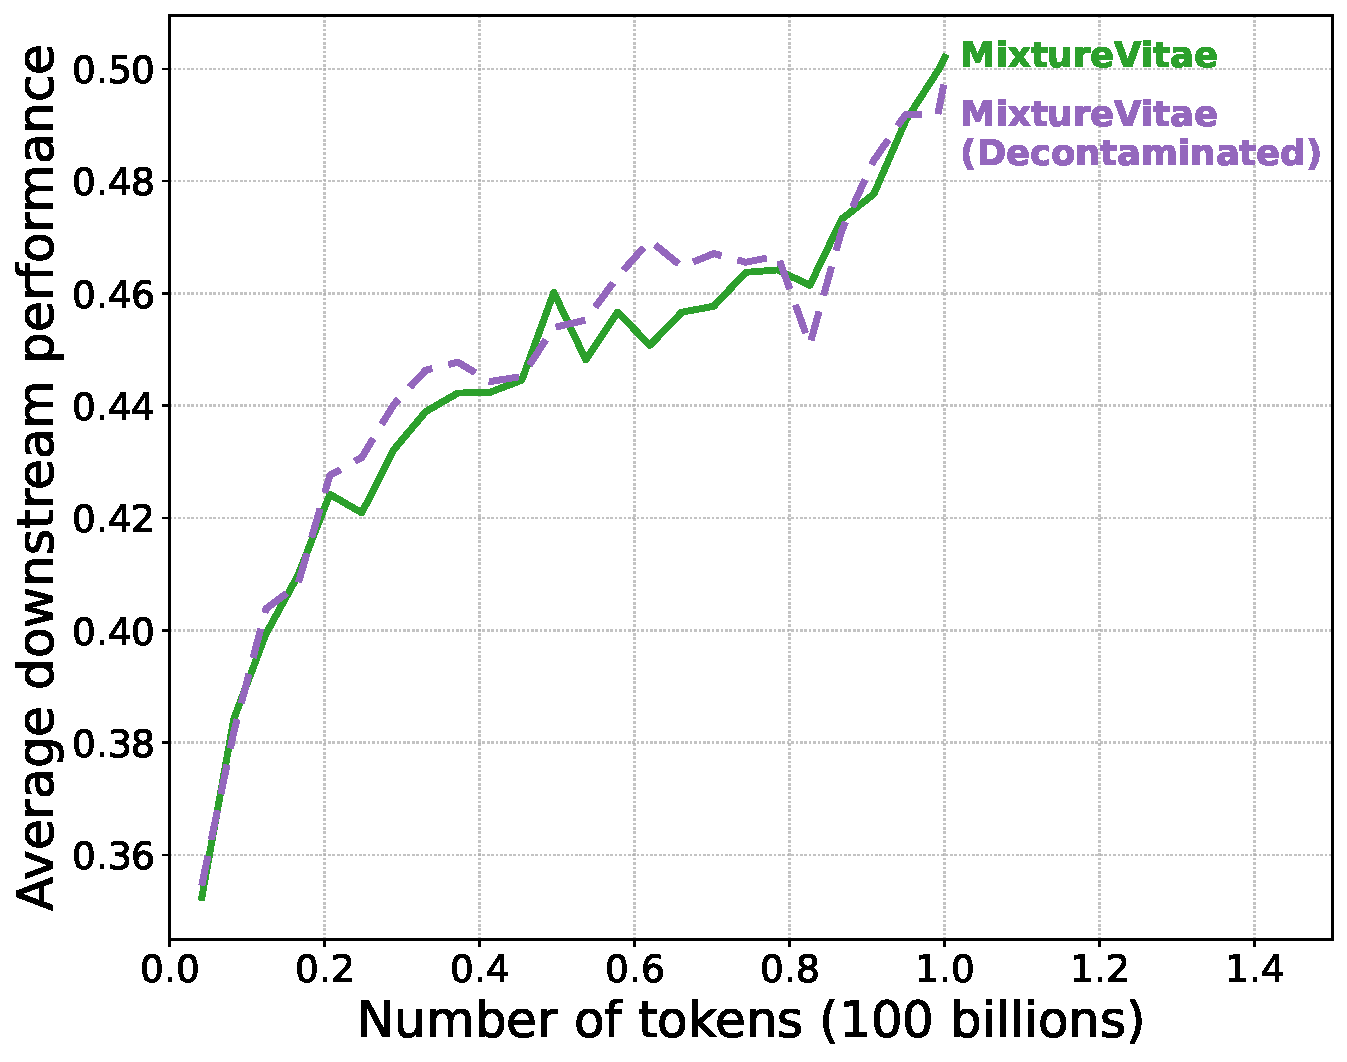
\includegraphics[width=0.95\linewidth]{figures/100B_perf_contam.pdf}
\caption{Average accuracy across all tasks (as listed in Table~\ref{tab:eval_settings_general}) as a function of number of training steps.}
\end{subfigure}%
     \begin{subfigure}[t]{0.48\textwidth}
        \centering        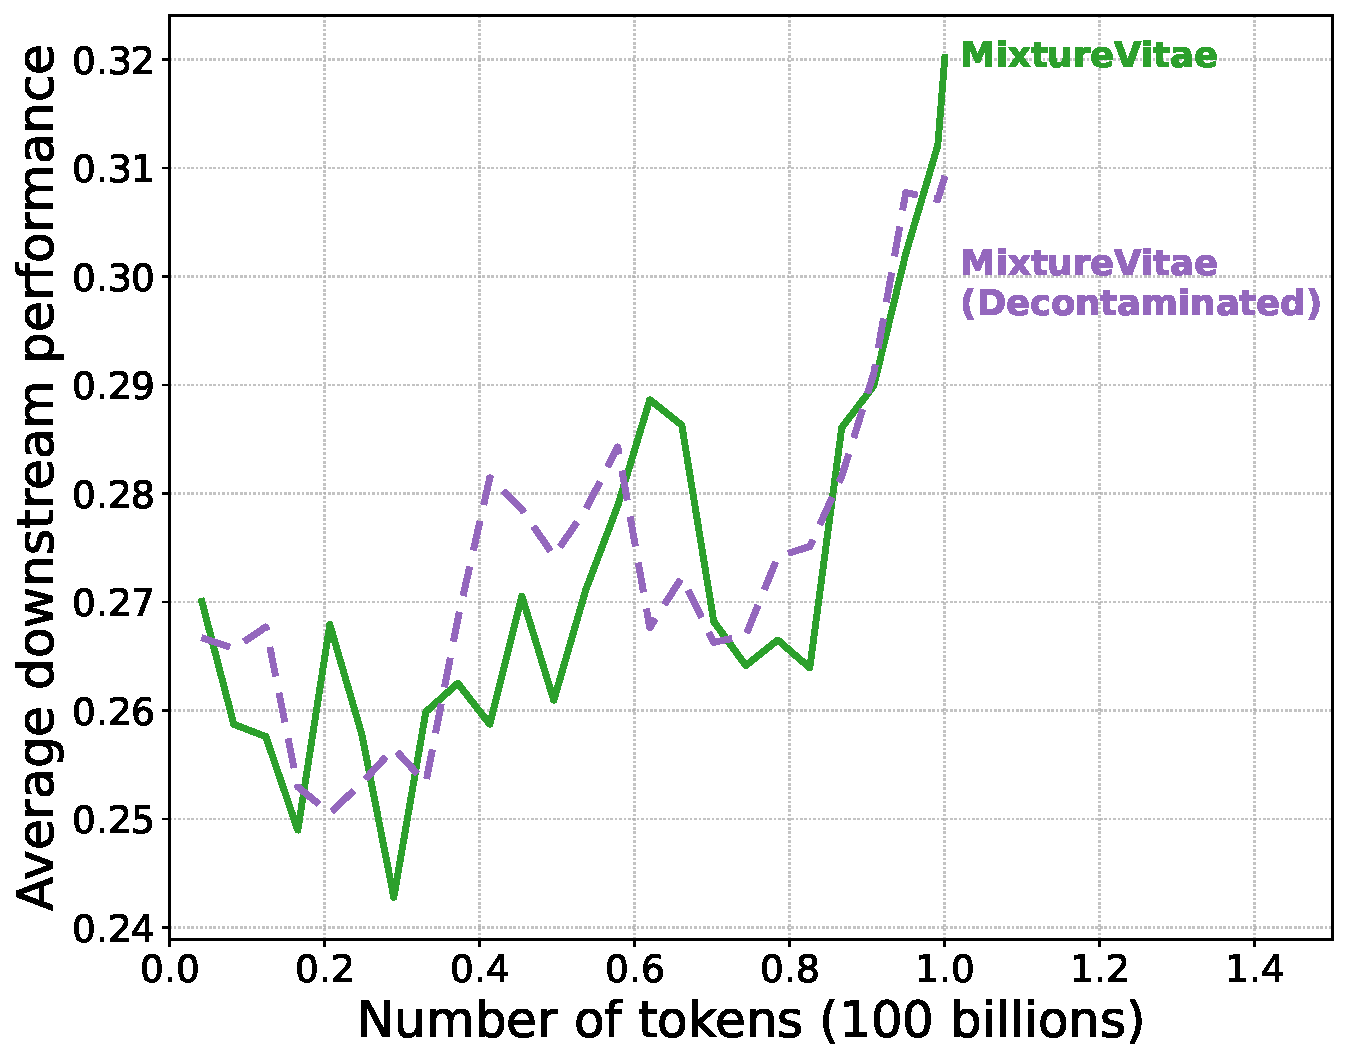
\includegraphics[width=0.95\linewidth]{figures/100B_perf_MMLU}
        \caption{Accuracy on MMLU as a function of number of training steps.}
        \label{fig:mmlu_contam}
    \end{subfigure}
  \caption{\textbf{Validation of 1.7B model performance}. The \textbf{\MixtureVitae{} (Decontaminated)} model (purple, dashed), trained with dataset shards responsible for benchmark leakage removed, performs closely to the full \MixtureVitae{} (green, solid) model. This confirms our results are not an artifact of test set leakage.}
  \label{fig:ablate_app}
\end{figure}

\textbf{D.5 Full Decontamination Experiment} \\
We also performed a stronger decontamination experiment in which we removed \emph{every} document in \MixtureVitae{} that was flagged as contaminated by our 13-gram procedure (Appendix~\ref{app:contam_report}) and retrained a 1.7B model for 300B tokens under the \texttt{open-sci-ref} setup. The results---shown in Figure~\ref{fig:full_decontam}---indicate that the fully decontaminated variant performs slightly \emph{better} than the original \MixtureVitae{} model, further addressing concerns that our benchmark results might be inflated by data leakage.

\begin{figure}[htb]
    \centering
    
\includegraphics[width=0.5\linewidth]{figures/300B_mxv_decontam.pdf}
    \caption{\textbf{1.7B model performance on a fully decontaminated dataset}. The model trained on the fully decontaminated \MixtureVitae{} corpus (purple, dashed) performs slightly better than the model trained on the full \MixtureVitae{} dataset (green, solid), further indicating that benchmark gains are not driven by contaminated examples.
 }
    \label{fig:full_decontam}
\end{figure}

\subsection{Discussion on Decontamination Methodology}
\label{app:decontam_discussion}

Our decontamination pipeline employs the standard 13-gram exact-match procedure~\citep{abdin2024phi4technicalreport} to ensure high precision, scalability and comparability with prior baselines. While we acknowledge that exact matching overlooks paraphrased content, we avoided approximate methods (e.g., LSH, embedding-based) due to their tendency to produce false positives on common factual or algorithmic templates \citep{lee2022deduplicating}. As noted in \citet{penedo2024}, aggressive removal of semantically similar content risks distorting the training distribution by discarding high-value instructional data.